\section{Background}
\label{sec:background}

We now outline how a CDN typically operates, including what information it
has access to. We also discuss some of the ongoing legal
questions that CDNs currently face.

\subsection{Content Delivery Networks}
CDNs cache content as a service to content publishers.  A 
content publisher may wish to use a CDN provider for several reasons:

\begin{itemize}[noitemsep]
\item CDNs cache content in geographically distributed locations, which allows for localized data centers, faster download speeds, and reduces the load on the content publisher's server.
\item CDNs typically provide usage analytics, which can help a content publisher get a better understanding of usage as compared to the publisher's understanding without a CDN.
\item CDNs provide a high capacity infrastructure, and therefore provide higher availability, lower network latency, and lower packet loss.  
\item CDNs' data centers have high bandwidth, which allows them to handle and mitigate DDoS attacks better than the content publisher's server.
\end{itemize}

CDN providers usually have a large number of edge servers that cache content;
for example, Akamai has more than 216,000 servers in over 120 countries around
the world~ \cite{akamai_facts}.  Having more edge servers in more locations
increases the probability that a cache is geographically close to a client,
which helps reduce the end-to-end latency, as well as the likelihood of
certain kinds of attacks, such as BGP (Border Gateway Protocol) hijacking.
When a client requests a web page, the closest edge server to the client that
contains the content is identified, and the content is served from that edge
server.  Most often, this edge server is geographically closer to the client
than the content publisher's server, thus allowing the client to retrieve the
content faster. If the requested page's content is not in one of the CDN's
caches, then the request is forwarded to the content publisher's server; the
CDN caches the response and returns the content to the client.

%\begin{figure}[t]
%\centering
%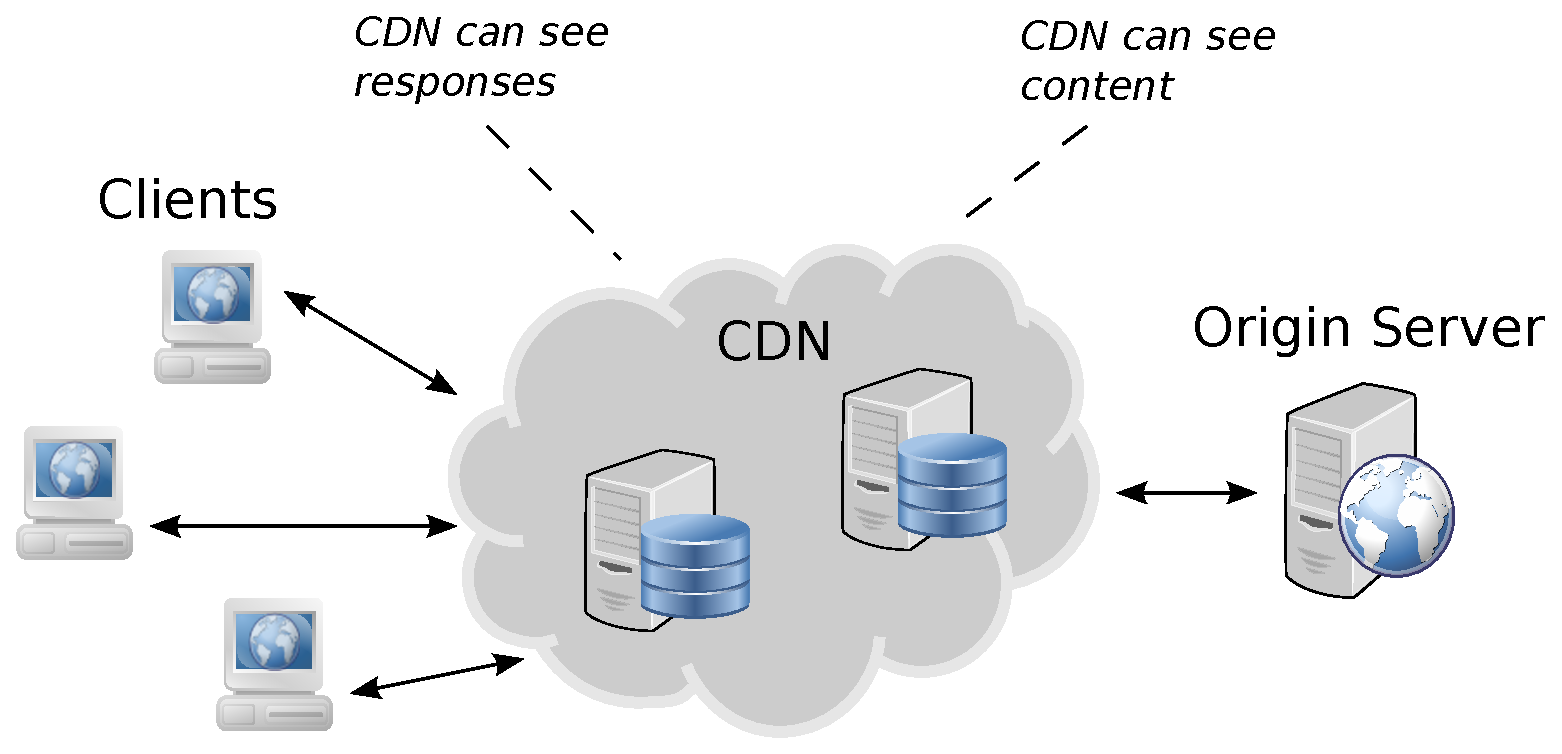
\includegraphics[width=.375\textwidth]{plain_cdn_new2}
%\caption{The relationships between clients, the CDN, and content publishers in 
%CDNs today.}
%\label{fig:basic_cdn}
%\end{figure}

\subsection{What CDNs Can See}
\label{sec:info}

Because the CDN interacts with both content publishers and clients%, as shown in Figure~\ref{fig:basic_cdn}
, it is in a unique position to learn an
enormous amount of information.  CDN providers know information about the content they serve, information about the clients who access data stored at the CDN, and information about all content publishers that cache content at CDN edge servers.

\textbf{Content.}  CDNs typically have access to all content that they distribute,
as well as 
the corresponding URL.  First, the CDN must use the URL, which is not 
encrypted or hidden, to locate and serve the content. Therefore, 
the CDN already knows what content is
stored in its caches.  Because CDNs provide analytics to content publishers, they
keep track of cache hit 
rates, and how often content is accessed.  The CDN not only knows
about the content identifier; it also also 
has access to the plaintext content in order to perform optimizations on the content
to increase performance (\eg, minimizing CSS, HTML, and JavaScript).  
They can also inspect content to upgrade a connection to HTTPS; we discuss how 
\system{} handles these types of optimizations
in Section \ref{sec:discussion}. In addition, requesting content via HTTPS does not hide any information 
from the CDN as the CDN terminates TLS connections on behalf of the 
content publisher.  This means that not only does the CDN know the content, the
content identifier, but also it knows 
public and private keys, as well as certificates associated with the content it caches.  

\textbf{Client information.} Clients retrieve content directly from the
CDN's edge servers. These requests reveal
information about the client's location and what the client is accessing.  
CDNs can also see each client's cross-site browsing patterns: CDNs host content
for
many different publishers, which allows 
them to see content requests for content published by different publishers.  Akamai caches enough content around the world to see up to 30\% of global Internet 
traffic~\cite{akamai_global_traffic}.  The implications of a CDN having access to
this much information was evident when Cloudflare
went public with the National Security Letters they had received~\cite{cloudflare_nsl};
these National Security Letters
demanded information collected by the CDN and also included a gag order, which prohibits
the CDN from publicly announcing the information request.  

\textbf{Content publisher information.} A CDN must know information
about their customers, the content
publishers; the CDN keeps track of who the content publisher is and 
what the publisher's content is.  The combination of the CDN seeing all content in plaintext and the content's 
linkability with the publisher, gives the CDN even more power.  Additionally, as mentioned previously, the CDN often 
holds the publisher's keys (including the private key), and the publisher's certificates.  This has led to doubts 
about the integrity of content because a CDN can impersonate the publisher from the client's point of view~\cite{levy2015stickler}.



\subsection{Open Legal Questions}
%  In the 
%copyright realm, the European Commission is considering legislation that would remove safe harbor protection against copyright law for 
%online service providers if they host infringing content, regardless of the provenance of that content. 

Various parties are battling in the courts over cases that pertain to user
data requests and intermediary liability.  Intermediary liability would impose
criminal liability on an Internet platform (or a CDN) for the content it
provides on behalf of its customers or users. In this section, we highlight
some of these cases, which point to a key problem that CDNs face: by knowing
all the content that they distribute, CDNs may be burdened with the legal
responsibility for the actions of their customers and clients.

\textbf{User Data Requests.}
There are numerous open questions in the legal realm regarding which government can request data stored in different countries, which 
has led to much uncertainty.  A series of recent events have illustrated this uncertainty.  In the struggle over government access to 
user data, cases such as {\it Microsoft vs. United States} (often known as the ``Microsoft Ireland Case'') concerns whether the United 
States Government should have access to data about U.S. citizens stored abroad, given that Microsoft is a U.S. corporation.  

Additionally, third parties have asked CDNs for user data.  The Cloudflare CDN has
been required
to share data with FBI~\cite{cloudflare_nsl}; similarly, leaked NSA documents showed
that the government agency ``collected information `by exploiting inherent 
weaknesses in Facebook's security model' through its use of the popular Akamai content
delivery network''~\cite{facebook_surv}.

\textbf{Intermediary Liability.}
More recently, questions on intermediary liability have been in the spotlight.  For example, many groups, including the Recording Industry 
Association of America (RIAA) and the Motion Picture Association of America (MPAA), have targeted CDNs with takedown notices for 
content that allegedly infringes on copyright, trademarks, and patent rights; CDNs are a more convenient target of these takedown notices than 
the content provider because oftentimes the content provider is either located in a jurisdiction where it is difficult to enforce the takedown, 
or it is difficult to determine the owner of the content \cite{medium_copyright,eff_copyright}.
Although Section 230 of the Communications Decency Act protects intermediaries,
such as CDNs, from being held
liable for the content they distribute, there have been cases where CDNs are forced
to remove content.  This happened in 2015 involving the RIAA, Cloudflare, and Grooveshark \cite{techdirt_copyright}. In 2017, a district court ruled that Cloudflare is not protected from anti-piracy injunctions by the Digital Millennium Copyright Act (DMCA)~\cite{stack_copyright}.

The role of a CDN as an intermediary has also come into question in recent legislation, including a 2017 German hate speech law~\cite{netenforementact} and a U.S. law known as FOSTA-SESTA~\cite{fosta_sesta}. Both laws raise the spectre of potentially holding CDNs liable for the content that they distribute, despite the CDN not being a party in the content publishing.

%In October 2017, Germany passed a new law that imposes large fines, upwards of five million euros, on social media companies that do not take down illegal, racist, or slanderous comments and posts within 24 hours.  The law targets companies such as Facebook, Google, and Twitter, but could also apply to smaller companies, which could be serviced by CDNs.  In the latter case, it is an open question whether this new law also applies to CDNs.  In the United States, the SESTA bill would make Internet platforms liable for their user's illegal comments and posts.  SESTA would hold CDNs liable for the content that they distribute (despite the CDN not being a party in the content publishing); these types of laws can naturally lead to overblocking, where an intermediary errs on the side of caution and censors more content than it needs to. Such a law may also set a precedent for the censoring other types of content that are unpopular but legal. 
